The telecommunication company Nett provides capacity between cites in Europe. The cities are Stockholm, Berlin, London, Warsaw, Paris, Madrid and Rome. Some of the cities are connected in which traffic can be sent in both directions. The connections and the maximum traffic which can be sent between the cites respectively can be seen in Figure 1.

Nett wishes to provide 50 Gbit/s between Stockholm and Rome at the same time they provide 40 Gbit/s between London and Warsaw. They need help in routing the traffic because of the capacity limitations. Also, they would like to investigate if there is any slack in the network, potential to adding another traffic route and how to handle fluctuations in capacity.

\begin{center}
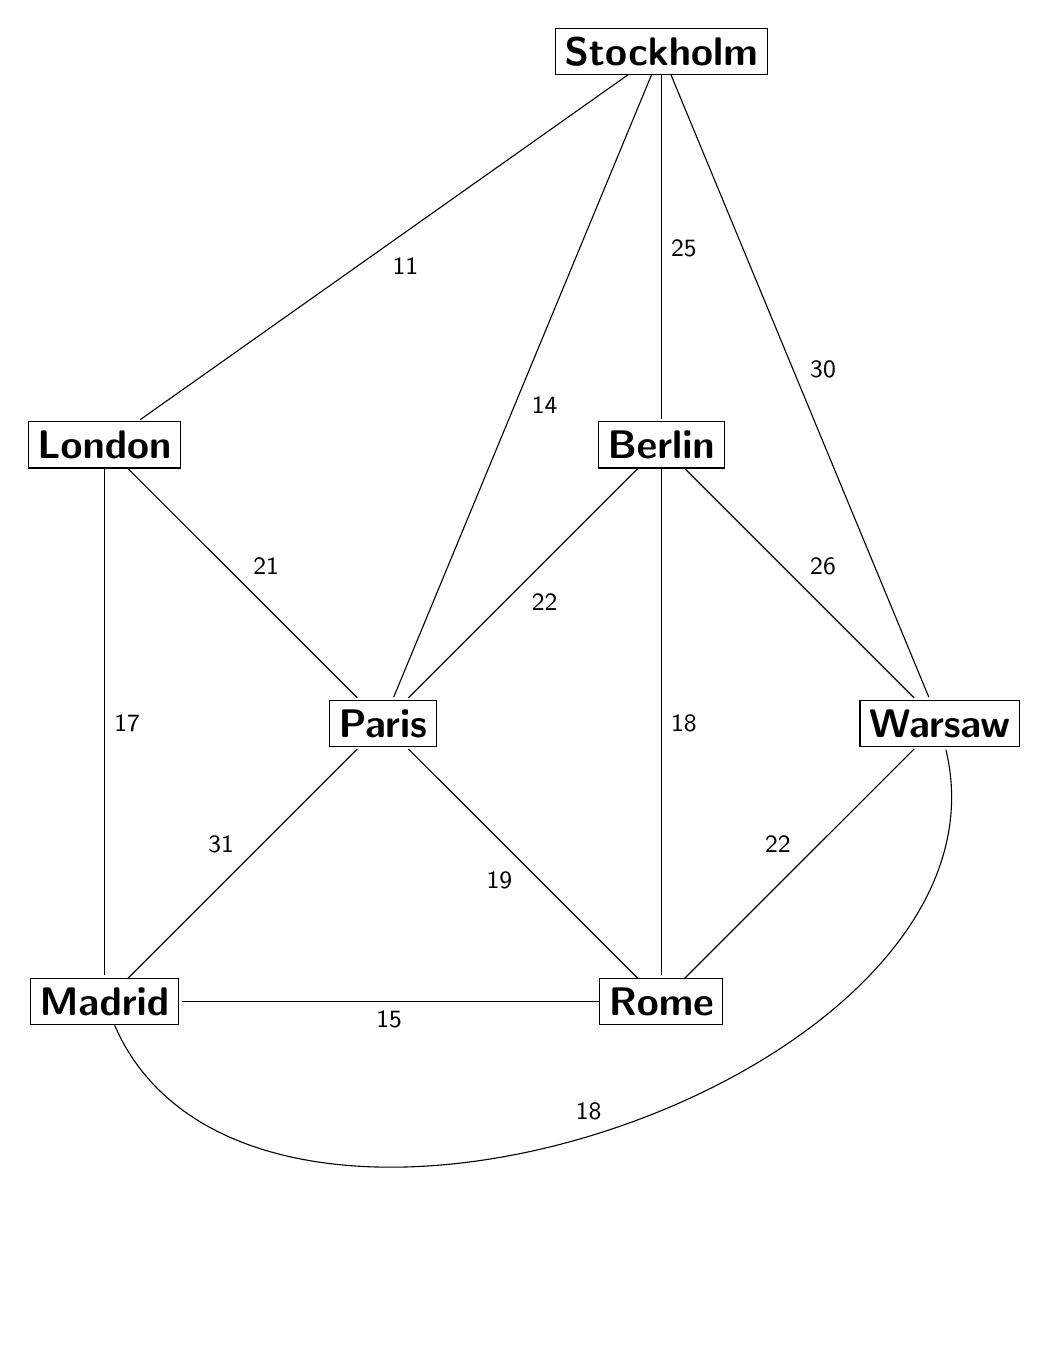
\begin{tikzpicture}[shorten >=1pt,auto,node distance=5cm,
                    main node/.style={rectangle,draw,font=\sffamily\Large\bfseries}]
  \node[main node] (1) {Stockholm};
  \node[main node] (2) [below of=1] {Berlin};
  \node[main node] (3) [below right of=2] {Warsaw};
  \node[main node] (4) [below left of=2] {Paris};
  \node[main node] (5) [above left of=4] {London};
  \node[main node] (6) [below right of=4] {Rome};
  \node[main node] (7) [below left of=4] {Madrid};

  \path[every node/.style={font=\sffamily\small}]
    (1) edge node {25} (2)
     	edge node {30} (3)
    	edge node {14} (4)
    	edge node {11} (5)
    (2) edge node {26} (3)
    	edge node {22} (4)
        edge node {18} (6)
    (5) edge node {17} (7)
        edge node {21} (4)
    (6) edge node {19} (4)
        edge node {15} (7)
        edge node {22} (3)
    (7) edge [bend right=85] node {18} (3)
    	edge node {31} (4);
  
\end{tikzpicture}
\end{center}
Figure 1. System modelled as a network where maximum capacity is marked out on the arcs.

\newpage

\section{Routing the traffic}
In this section we investigate the best way to sent the traffic in the network. 50Gbit/s must be sent from Stockholm to Rome at the same time 40Gbit/s is sent from London to Warsaw without violating the capacity limitations. We would like to spread the traffic evenly. Therefore, we minimize the strain on any link in the network, i.e. traffic divided by the capacity.

\subsection{Mathematical formulation}
To solve this we treat the cities and links as a network and the traffic as a flow throughout the network. The cities are nodes connected by links which are arcs. Stockholm is a source node where 50Gbit/s comes in which will be distributed to the sink node Rome. The same goes for London and Warsaw respectively.

We start by introduction the set $I$ :
$$I = \{ Sto,Lon,Ber,War,Par,Rom,Mad\}$$

The set $I$ make up for the network's node and an arc between node $i$ and $j$ is denoted as ($i$,$j$). The flows from Stockholm and London can be sent in the same link in either direction. However, the two flows must be treated independently. That being said, the 50Gbit/s that comes in from Stockholm is the same 50Gbit/s that arrives at Rome. We must keep track of the flows which is why we introduce another index k. The flow from Stockholm to Rome is $k=1$ and the flow from London to Warsaw is $k=2$.

For each arc in the network, there will be a corresponding variable $x_{i,j,k}$ which denotes the flow from node $i$ to $j$ of flow $k$. Solving for the variable $x$ will provide the strategy for how to send the traffic between the cites. Though, there are two constraints which must be taken into account. 

The first constraint deals with conservation of flow, i.e. the flow into a node is equal the flow out.
$$\sum\limits_{j \in I} x_{i,j,k} - \sum\limits_{j \in I} x_{j,i,k} = b_{i}$$

$$
\text{where } b_{i} = 
 \begin{bmatrix}
  b_{Sto}\\
  b_{Ber}\\
  b_{War}\\
  b_{Lon}\\
  b_{Par}\\
  b_{Mad}\\
  b_{Rom}
 \end{bmatrix} =
 \begin{bmatrix}
  50\\
  0\\
  -40\\
  40\\
  0\\
  0\\
  -50
 \end{bmatrix}
$$


The other constraint is that both types of traffic, in either direction, must not exceed the capacity in each link. If there is no direct connections between two cities, the capacity is zero and no traffic can be sent in this arc.
$$\sum\limits_{k =1}^2 x_{i,j,k} + \sum\limits_{k =1}^2 x_{j,i,k} \leq c_{i,j}\\$$

$$
\text{where $c_{i,j}$ is the maximum capacity in arc (i,j)}$$

Finally, we define the objective function as the utility in a link.

$$\frac{\sum\limits_{k =1}^2 x_{i,j,k} + \sum\limits_{k =1}^2 x_{j,i,k}}{c_{i,j}}$$

Taking all the above into consideration, the mathematical formulation of the network flow optimization problem becomes:

$$
\begin{tabular}{r c l}
		min & $\frac{\sum\limits_{k =1}^2 x_{i,j,k} + \sum\limits_{k =1}^2 x_{j,i,k}}{c_{i,j}}$\\
		s.t. & $\sum\limits_{j \in I} x_{i,j,k} - \sum\limits_{j \in I} x_{j,i,k} = b_{i}$\\
		& $\sum\limits_{k =1}^2 x_{i,j,k} + \sum\limits_{k =1}^2 x_{j,i,k} \leq c_{i,j}$\\
		& $x_{i,j,k} \geq 0\quad \forall \: i,j \in I$
	\end{tabular}
$$

\subsection{Result}
\begin{center}
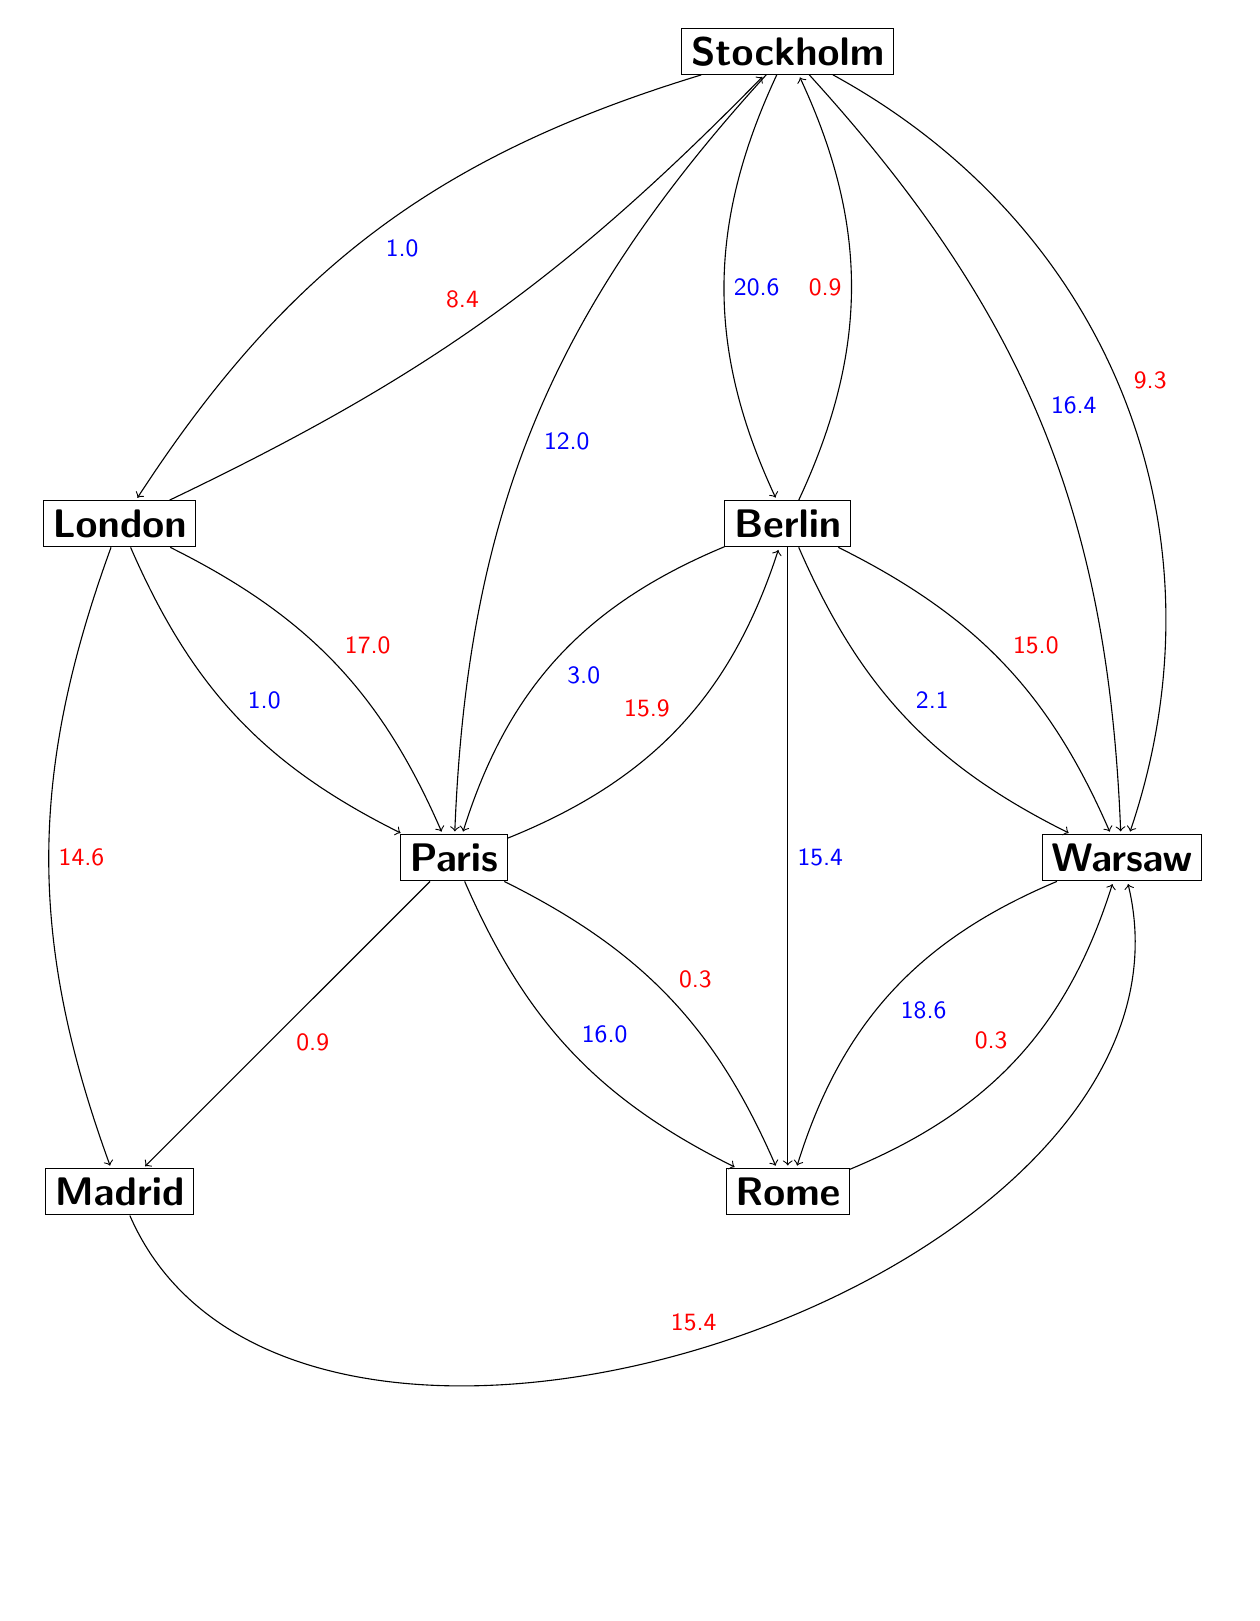
\begin{tikzpicture}[->,shorten >=1pt,auto,node distance=6cm,
                    main node/.style={rectangle,draw,font=\sffamily\Large\bfseries}]
  \node[main node] (1) {Stockholm};
  \node[main node] (2) [below of=1] {Berlin};
  \node[main node] (3) [below right of=2] {Warsaw};
  \node[main node] (4) [below left of=2] {Paris};
  \node[main node] (5) [above left of=4] {London};
  \node[main node] (6) [below right of=4] {Rome};
  \node[main node] (7) [below left of=4] {Madrid};

  \path[every node/.style={font=\sffamily\small}]
    (1) edge [bend right=20] node[blue] {1.0} (5)
    	edge [bend right=20] node[blue] {12.0} (4)
     	edge [bend right=25] node[blue] {20.6} (2)
    	edge [bend left=20] node[blue] {16.4} (3)
    	edge [bend left=40] node[red] {9.3} (3)
    (2) edge [bend right=25] node[red] {0.9} (1)
    	edge [bend right=25] node[blue] {3.0} (4)
        edge [bend right=20] node[blue] {2.1} (3)
    	edge [bend left=20] node[red] {15.0} (3)
    	edge node[blue] {15.4} (6)
    (3) edge [bend right=25] node[blue] {18.6} (6)
    (4) edge [bend right=25] node[red] {15.9} (2)
    	edge [bend right=20] node[blue] {16.0} (6)
    	edge [bend left=20] node[red] {0.3} (6)
    	edge node[red] {0.9} (7)
    (5) edge [bend right=10] node[red] {8.4} (1)
    	edge [bend left=20] node[red] {17.0} (4)
    	edge [bend right=20] node[blue] {1.0} (4)
		edge [bend right=20] node[red] {14.6} (7)
	(6) edge [bend right=25] node[red] {0.3} (3)
    (7) edge [bend right=85] node[red] {15.4} (3);
  
\end{tikzpicture}
\end{center}